\documentclass[footinclude=false,11pt,DIV11]{scrartcl}

% Wenzel's standard prelude
% ----- 8< ----- 8< ------

\usepackage[english]{babel}
\usepackage[T1]{fontenc}
\usepackage[utf8]{inputenc}
\usepackage{graphicx}
\usepackage{amsmath}
\usepackage{mathtools}
\usepackage{array}
\usepackage{booktabs}
\usepackage{tabularx}
\usepackage{color}
\usepackage{colortbl}
\usepackage{listings}
\usepackage{enumerate}
\usepackage{upquote}
\usepackage[absolute]{textpos} % Manual placement of certain things
\usepackage{ragged2e} % Ragged-right columns with hyphenation
\usepackage{nicefrac}
\usepackage{macros}
\usepackage[format=hang,font=small,labelfont=bf]{caption}
\usepackage[expansion=false, babel=true]{microtype}
\usepackage{subfig}

% Make sure that ligatures remain searchable in the PDF
\input glyphtounicode
\pdfgentounicode=1

\IfFileExists{MinionPro.sty}
   {\usepackage[opticals,fullfamily,lf]{MinionPro}}
      {\message{Package MinionPro.sty was not found.}}

\setcounter{secnumdepth}{3}
\setcounter{tocdepth}{3}

\newcommand{\MitsubaVersion}{0.3.0}

\typearea[current]{last}
\raggedbottom
\renewcommand*\ttdefault{txtt}

\usepackage{scrpage2}
\ofoot[]{}
\cfoot[]{}
\automark[subsection]{section}
\ihead{\sc\leftmark}
\ohead{\sc\rightmark}
\chead{}
\setheadsepline{.2pt}
\setkomafont{pagenumber}{\normalfont}
\addtokomafont{sectioning}{\color{myblue}\rmfamily}
\addtokomafont{descriptionlabel}{\rmfamily}
\pagestyle{scrheadings}

\usepackage[
	bookmarks,
	bookmarksnumbered,
	colorlinks,
	plainpages=false,
	pdfpagelabels,
	hypertexnames=false,
	linkcolor=myblue,
	urlcolor=myblue,
	citecolor=myblue,
	pdfpagelabels,
	pdftitle={Mitsuba \MitsubaVersion\, Documentation},
	pdfauthor={Wenzel Jakob},
	pdfstartview=FitH
]{hyperref}

\definecolor{myblue}{rgb}{0,.1,.6}
\definecolor{myred}{rgb}{0.63,.16,.16}
\definecolor{lstshade}{gray}{0.95}
\definecolor{lstframe}{gray}{0.80}
\definecolor{lstcomment}{gray}{0.5}
\definecolor{lstattrib}{rgb}{0,0.34,0}

% Listings settings
\lstset{
	basicstyle = \small\ttfamily\raggedright,
	mathescape = true,
	frame = lrtb,
	backgroundcolor = \color{lstshade},
	rulecolor = \color{lstframe},
	tabsize = 4,
	columns = flexible,
	keepspaces,
	belowskip = \smallskipamount,
	framerule = .7pt,
	breaklines = true,
	showstringspaces = false,
	keywordstyle = \bfseries,
	captionpos = b,
	upquote = true
}

\lstdefinelanguage{xml} {
	sensitive=true,
	morecomment=[s][\color{lstcomment}\itshape]{<!--}{-->},
	morecomment=[s][\color{lstcomment}]{<?}{?>},
	string=[b]", stringstyle=\color{lstattrib},
	keywords= [1] {
		shape,bsdf,scene,texture,phase,integer,float,
		string,transform,ref,rgb,srgb,spectrum,blackbody,
		medium,camera,film,sampler,integrator,luminaire,
		translate,rotate,scale,lookAt,point,vector,matrix,
		include,fscat
	},
}

% Set up textpos
\TPGrid{68}{108}

% Thick frames for images
\setlength\fboxsep{0pt}
\setlength\fboxrule{1.5pt}

% Less vertical spacing for \figure[h] floats
\setlength{\intextsep}{3pt}

\lstnewenvironment{shell}[1][]{\lstset{#1}}
	{}
\lstnewenvironment{cpp}[1][]{\lstset{language=c++, #1}}
	{}
\lstnewenvironment{xml}[1][]{\lstset{language=xml, #1}}
	{}
\lstnewenvironment{console}[1][]{\lstset{basicstyle=\footnotesize\ttfamily, float, #1}}
	{}

% ----- 8< ----- 8< ------

\title{
	Mitsuba Documentation\\\vspace{3mm}
	\large Version \MitsubaVersion
}
\author{Wenzel Jakob}
\date{\today}

\begin{document}
\maketitle
\clearpage
\ofoot[\pagemark]{\pagemark}

\tableofcontents

\part{Using Mitsuba}
\textbf{Disclaimer:} This is manual documents the usage, file format, and
internal design of the Mitsuba rendering system. It is currently a work
in progress, hence some parts may still be incomplete or missing.

\section{About Mitsuba}
Mitsuba is a research-oriented rendering system in the style of PBRT
(\url{www.pbrt.org}), from which it derives much inspiration.
It is written in portable C++, implements unbiased as well
as biased techniques, and contains heavy optimizations targeted
towards current CPU architectures.
Mitsuba is extremely modular: it consists of a small set of core libraries
and over 100 different plugins that implement functionality ranging
from materials and light sources to complete rendering algorithms.

In comparison to other open source renderers, Mitsuba places a strong
emphasis on experimental rendering techniques, such as path-based
formulations of Metropolis Light Transport and volumetric
modeling approaches. Thus, it may be of genuine interest to those who
would like to experiment with such techniques that haven't yet found
their way into mainstream renderers, and it also provides a solid
foundation for research in this domain.

Other design considerations are:

\parheader{Performance:}
Mitsuba provides optimized implementations of the most commonly
used rendering algorithms. By virtue of running on a shared foundation, comparisons between them can
better highlight the merits and limitations of different approaches. This is in contrast to, say,
comparing two completely different rendering products, where technical information on the underlying
implementation is often intentionally not provided.

\parheader{Robustness:}
In many cases, physically-based rendering packages force the user to model scenes with the underlying
algorithm (specifically: its convergence behavior) in mind. For instance, glass windows are routinely
replaced with light portals, photons must be manually guided to the relevant parts of a scene, and
interactions with complex materials are taboo, since they cannot be importance sampled exactly.
One focus of Mitsuba will be to develop path-space light transport algorithms, which handle such
cases more gracefully.

\parheader{Scalability:} Mitsuba instances can be merged into large clusters, which transparently distribute and
jointly execute tasks assigned to them using only node-to-node communcation. It has successfully
scaled to large-scale renderings that involved more than 1000 cores working on a single image.
Most algorithms in Mitsuba  are written using a generic parallelization layer, which can tap
into this cluster-wide parallelism. The principle is that if any component of the renderer produces
work that takes longer than a second or so, it at least ought to use all of the processing power
it can get.

The renderer also tries to be very conservative in its use of memory, which allows it to handle
large scenes (>30 million triangles) and multi-gigabyte heterogeneous volumes on consumer hardware.

\parheader{Realism and accuracy:} Mitsuba comes with a large repository of physically-based
reflectance models for surfaces and participating media. These implementations
are designed so that they can be used to build complex shader networks, while
providing enough flexibility to be compatible with a wide range of different
rendering techniques, including path tracing, photon mapping, hardware-accelerated rendering
and bidirectional methods.

The unbiased path tracers in Mitsuba are battle-proven and produce
reference-quality results that can be used for predictive rendering, and to verify
implementations of other rendering methods.

\parheader{Usability:}
Mitsuba comes with a graphical user interface to interactively explore scenes. Once a suitable
viewpoint has been found, it is straightforward to perform renderings using any of the
implemented rendering techniques, while tweaking their parameters to find the most suitable
settings. Experimental integration into Blender 2.5 is also available.

\section{Limitations}
Mitsuba can be used to solve many interesting light transport problems.
However, there are some inherent limitations of the system that users should be aware of:
\begin{enumerate}[(i)]
\item \textbf{Wave Optics}: Mitsuba is fundamentally based on the geometric optics toolbox,
which means that it generally does not simulate phenomena that arise due to
the wave properties of light (diffraction, for instance).
\item \textbf{Polarization}: Mitsuba does not account for polarization. In
other words, light is always assumed to be randomly polarized. This can be a problem for
some predictive rendering applications.
\item \textbf{Numerical accuracy}: The accuracy of any result produced with this
system is constrained by the underlying floating point computations.

For instance, an intricate scene that can be rendered without problems,
may produce the wrong answer when all objects are translated away from the
origin by a large distance, since floating point numbers are spaced less densely at the
new position.  To avoid these sorts of pitfalls, it is good to have a basic
understanding of the IEEE-754 standard.
\end{enumerate}

\section{License}
Mitsuba is free software and can be redistributed and modified under the terms of the GNU General
Public License (Version 3) as provided by the Free Software Foundation.

\remarks{
	\item Being a ``viral'' license, the GPL automatically applies to all
	derivative work. Amongst other things, this means that without express
	permission, Mitsuba's source code is \emph{off-limits} to companies that
	develop rendering software not distributed under a compatible license.
}

\section{Compiling the renderer}
To compile Mitsuba, you will need a recent C++ compiler (e.g. GCC 4.1+ or 
Visual Studio 2005+) and some additional libraries, which Mitsuba uses internally. 
Builds on all three supported platforms are done using a unified system
based on SCons (\url{http://www.scons.org}), a flexible python-based 
software construction tool. There are some minor differences between operating systems though: for
more details, please refer to one of the next sections depending on which one you use.

\subsection{Common steps}
To get started, you will need to download a recent version of Mitsuba: make sure that you have the Mercurial (\url{http://mercurial.selenic.com/})
versioning system installed and enter the following at the command prompt:
\begin{shell}
$\texttt{\$}$ hg clone https://www.mitsuba-renderer.org/hg/mitsuba
\end{shell}
On Windows, you can instead use the more convenient TortoiseHG shell extension (\url{http://tortoisehg.bitbucket.org/}) 
to do this directly from the Explorer.

Common to all platforms is that a build configuration file must be chosen: amongst the
following, please copy the best matching file into a new file to the root of the Mitsuba
directory and rename it into \code{config.py}.
\begin{shell}
config/config-linux.py  
config/config-darwin-x86_64.py  
config/config-darwin-x86.py  
config/config-darwin-universal.py  
config/config-msvc2005-win32.py  
config/config-msvc2005-win64.py
\end{shell}

Some minor adjustments may have to be made to this file based on your configuration. 
You may also set adjust certain compilation flags here:
\begin{description}
\item[\texttt{MTS\_DEBUG}] Enable assertions etc. Usually a good idea.
\item[\texttt{SINGLE\_PRECISION}] Do all computation in single precision. This is usually sufficient.
\item[\texttt{DOUBLE\_PRECISION}] Do all computation in double precision. Incompatible with
\texttt{MTS\_SSE}, \texttt{MTS\_HAS\_COHERENT\_RT}, and \texttt{MTS\_DEBUG\_FP}.
\item[\texttt{MTS\_SSE}]Activate optimized SSE routines.
\item[\texttt{MTS\_HAS\_COHERENT\_RT}]Include coherent ray tracing support (depends on \texttt{MTS\_SSE}).
\item[\texttt{MTS\_DEBUG\_FP}]Generated NaNs will cause floating point exceptions, which can be caught in a debugger. Warning: This is slow!
\end{description}
All default configurations use the flags \code{MTS\_DEBUG}, \code{SINGLE\_PRECISION}, \code{MTS\_SSE}, \code{MTS\_HAS\_COHERENT\_RT}.
Initially, it is a good idea to just leave the configuration the way it is.

\subsection{Building on Ubuntu Linux}
You'll first need to install a number of dependencies. It is assumed here
that you are using Ubuntu Linux, hence some of the package may be named differently if you are 
using another distribution.

First, run
\begin{shell}
$\text{\$}$ apt-get install build-essential scons qt4-dev-tools scons libpng12-dev libjpeg62-dev libilmbase-dev libopenexr-dev libxerces-c2-dev libboost-dev libglewmx1.5-dev libxxf86vm-dev libboost-system-dev libboost-filesystem-dev
\end{shell}
To get COLLADA support, you will also need to install the \texttt{collada-dom} packages or build them from scratch. Here, we install the \code{x86\_64} binaries and development headers included with Mitsuba:
\begin{shell}
$\text{\$}$ dpkg --install tools/linux/collada-dom2.2_2.2-1_amd64.deb tools/linux/collada-dom-dev_2.2-1_amd64.deb
\end{shell}
Afterwards, simply run
\begin{shell}
$\text{\$}$ scons
\end{shell}
inside the Mitsuba directory. In the case that you have multiple processors, you might want to parallelize the build by appending \code{-j }\emph{core count} to the command.
If all goes well, SCons should finish successfully within a few minutes:
\begin{shell}
scons: $\texttt{done}$ building targets.
\end{shell}
To be able to run the renderer from the command line, you will also have to import it into your path:
\begin{shell}
$\text{\$}$ . setpath.sh
\end{shell}
(note the period at the beginning -- this assumes that you are using \code{bash}).

\subsection{Building on Fedora Core}
You'll first need to install a number of dependencies. It is assumed here
that you are using Fedora Core, hence some of the package may be named differently if you are 
using another distribution.

First, run
\begin{shell}
$\text{\$}$ yum install mercurial gcc-c++ boost-devel qt4-devel OpenEXR-devel xerces-c-devel
\end{shell}
You will also need the \texttt{glew-mx} and \texttt{collada-dom} packages, which are not included in the Fedora package repository. You can grab source and \texttt{i386} binary \texttt{RPM} files here: \texttt{http://www.mitsuba-renderer.org/release}.
Afterwards, simply run
\begin{shell}
$\text{\$}$ scons
\end{shell}
inside the Mitsuba directory. In the case that you have multiple processors, you might want to parallelize the build by appending \code{-j }\emph{core count} to the command.
If all goes well, SCons should finish successfully within a few minutes:
\begin{shell}
scons: $\texttt{done}$ building targets.
\end{shell}
To be able to run the renderer from the command line, you will also have to import it into your path:
\begin{shell}
$\text{\$}$ . setpath.sh
\end{shell}
(note the period at the beginning -- this assumes that you are using \code{bash}).


\subsection{Building on Windows}
This section assumes that Visual Studio 2008 is installed, but the instructions should work equally well with other versions.
On the Windows platform, Mitsuba already includes most of the dependencies in precompiled form.
You will still need to set up a few things though: first, you need to install Python 
(\url{www.python.org}) and SCons (\url{http://www.scons.org}) and ensure that they are contained
in the \code{\%PATH\%} environment variable so that entering \code{scons} on the command prompt
(\code{cmd.exe}) launches the build system (it will complain about not finding a project file though).
\begin{shell}
C:\Users\Wenzel>scons
scons: ** No SConstruct file found.
\end{shell}
\emph{Note: }On some setups, the SCons installer generates a warning about not finding Python in the registry. In this case, you can instead run \code{python setup.py install} within the source release of SCons.
Next, install Qt (\url{http://qt.nokia.com/downloads/windows-cpp-vs2008} -- you should get the release for Visual Studio 2008). Again, you need to make sure that the 
Qt utilities are reachable through the \code{\%PATH\%} environment variable so that you can for example launch \code{moc.exe} from the command line.

Because the official release of Qt currently only contains 32-bit binaries, you will accordingly have to 
build Mitsuba in 32-bit mode (i.e. you should use the configuration file \code{config-msvc2005-win32.py}). If you would rather like compile it in 64-bit mode, you have to create
your own 64-bit Qt binaries.

Having installed these dependencies, run the ``Visual Studio 2008 Command 
Prompt'' from the Start Menu (pick the \code{x86} version if you have the choice beetween \code{x86} and \code{x64}). Afterwards,
navigate to the Mitsuba directory and run \code{scons}. 
In the case that you have multiple processors, you might want to parallelize the build by appending \code{-j }\emph{core count} to the \code{scons} command.

If all goes well, the build process will finish successfully after a few
minutes. In comparison to the other platforms, you don't have to run the \code{setpath.sh} script at this point. 
All binaries are now located in the \code{dist} directory, and they should be executed directly from there.

\subsection{Building on Mac OS X}
On Mac OS X, you will need to install both scons (\code{www.scons.org}) and 
a recent release of XCode. You will also need to get Qt 4.7.0 Beta 2 or a newer version.
As of this writing, 4.7.0 Beta 2 is still the most recent release and can be found here: \url{http://qt.nokia.com/developer/qt-qtcreator-prerelease#download}
--- make sure that you get the normal Cocoa release (i.e. \emph{not} the one based on Carbon). All of the
other dependencies are already included in precompiled form.

Now open a Terminal and run
\begin{shell}
$\text{\$}$ scons
\end{shell}
inside the Mitsuba directory. In the case that you have multiple processors, you might want to parallelize the build by appending \code{-j }\emph{core count} to the command.
If all goes well, SCons should finish successfully within a few minutes:
\begin{shell}
scons: $\texttt{done}$ building targets.
\end{shell}
To be able to run the renderer from the command line, you will have to import it into your path:
\begin{shell}
$\text{\$}$ . setpath.sh
\end{shell}
(note the period at the beginning -- this assumes that you are using \code{bash}).

\section{Basic usage}
\label{sec:basics}
The rendering functionality of Mitsuba can be accessed through
a command line interface and an interactive Qt-based frontend. This section
provides some basic instructions on how to use them.
\subsection{Interactive frontend}
To launch the interactive frontend, run \code{Mitsuba.app} on MacOS, 
\code{mtsgui.exe} on Windows, and \code{mtsgui} on Linux (after sourcing \code{setpath.sh}).
You can also drag and drop scene files onto the application icon or the running program to open them.
A quick video tutorial on using the GUI can be found here: \url{http://vimeo.com/13480342}.
\subsection{Command line interface}
\label{sec:mitsuba}
The \texttt{mitsuba} binary is an alternative non-interactive rendering 
frontend for command-line use and batch job operation.
To get a listing of the parameters it supports, run
the executable without parameters:
\begin{shell}
$\texttt{\$}$ mitsuba 
\end{shell}
\lstref{mitsuba-cli} shows the output resulting from this command. The most common
mode of operation is to render a single scene, which is provided as a parameter, e.g.
\begin{shell}
$\texttt{\$}$ mitsuba path-to/my-scene.xml
\end{shell}
It is also possible to connect to network render nodes, which essentially lets Mitsuba parallelize
over additional cores. To do this, pass a semicolon-separated list of machines to 
the \code{-c} parameter. 
\begin{shell}
$\texttt{\$}$ mitsuba -c machine1;machine2;... path-to/my-scene.xml
\end{shell}
There are two different ways in which you can access render nodes:
\begin{itemize}
\item\textbf{Direct}: Here, you create a direct connection to a running \code{mtssrv} instance on
another machine (\code{mtssrv} is the Mitsuba server process). From the the performance 
standpoint, this approach should always be preferred over the SSH method described below when there is 
a choice between them. There are some disadvantages though: first, you need to manually start
\code{mtssrv} on every machine you want to use. 

And perhaps more importantly: the direct communication
protocol makes no provisions for a malicious user on the remote side. It is too costly
to constantly check the communication stream for illegal data sequences, so Mitsuba simply doesn't do it.
The consequence of this is that you should only use the direct communication approach within
trusted networks.

For direct connections, you can specify the remote port as follows:
\begin{shell}
$\texttt{\$}$ mitsuba -c machine:1234 path-to/my-scene.xml
\end{shell}
When none is given, Mitsuba assumes that the server uses default port 7554. 
\item \textbf{SSH}: 
    This approach works as follows: The renderer creates a SSH connection 
	to the remote side, where it launches a Mitsuba worker instance.
	All subsequent communication then passes through the encrypted link. 
	This is completely secure but slower due to the encryption overhead.
	If you are rendering a complex scene, there is a good chance that it
	won't matter much since most time is spent doing computations rather than
	communicating

	Such an SSH link can be created simply by using a slightly different syntax:
\begin{shell}
$\texttt{\$}$ mitsuba -c username@machine path-to/my-scene.xml
\end{shell}
	The above line assumes that the remote home directory contains
	a Mitsuba source directory (with compiled binaries) named \code{mitsuba}.
	If that is not the case, you need to provide the path to such a directory manually, e.g:
\begin{shell}
$\texttt{\$}$ mitsuba -c username@machine:/opt/mitsuba path-to/my-scene.xml
\end{shell}
	For the SSH connection approach to work, you \emph{must} enable passwordless 
	authentication.
	Try opening a terminal window and running the command \code{ssh username@machine} 
	(replace with the details of your remote connection).
	If you are asked for a password, something is not set up correctly --- please see 
	\url{http://www.debian-administration.org/articles/152} for instructions.

	On Windows, the situation is a bit more difficult since there is no suitable SSH client by
	default. To get SSH connections to work, Mitsuba requires \code{plink.exe} (from PuTTY) to
	be on the path. For passwordless authentication with a Linux/OSX-based
	server, convert your private key to PuTTY's format using \code{puttygen.exe}.
	Afterwards, start \code{pageant.exe} to load and  authenticate the key. All 
	of these binaries are available from the PuTTY website, and there is also
	a copy in the \code{tools/windows/bin}
	directory in the Mitsuba repository.

	It is possible to mix the two approaches to access some machines directly and others
	over SSH.
\end{itemize}
When doing many network-based renders over the command line, it can become tedious to
specify the connections every time. They can alternatively be loaded from a text file
where each line contains a separate connection description as discussed previously:
\begin{shell}
$\texttt{\$}$ mitsuba -s servers.txt path-to/my-scene.xml
\end{shell}
where \code{servers.txt} e.g. contains
\begin{shell}
user1@machine1.domain.org:/opt/mitsuba
machine2.domain.org
machine3.domain.org:7346
\end{shell}
\subsubsection{Passing parameters}
Any attribute in the scene XML file can be parameterized from the
command line.
For instance, you can render a scene several times with different reflectance values
on a certain material by changing its description to something like 
\begin{xml}
<bsdf type="lambertian">
	<spectrum name="reflectance" value="$\texttt{\$}$reflectance"/>
</bsdf>
\end{xml}
and running Mitsuba as follows:
\begin{shell}
$\texttt{\$}$ mitsuba -Dreflectance=0.1 -o ref_0.1.exr scene.xml 
$\texttt{\$}$ mitsuba -Dreflectance=0.2 -o ref_0.2.exr scene.xml 
$\texttt{\$}$ mitsuba -Dreflectance=0.5 -o ref_0.5.exr scene.xml 
\end{shell}

\subsubsection{Writing partial images to disk}
When doing lengthy command line renders on Linux or OSX, it is possible 
to send a signal to the process using 
\begin{shell}	
$\texttt{\$}$ killall -HUP mitsuba
\end{shell}
This causes the renderer to write out the partially finished 
image, after which it continues rendering. This can sometimes be useful to 
check if everything is working correctly.

\subsubsection{Rendering an animation}
The command line interface is ideally suited for rendering large amounts of files in batch
operation. You can simply pass in the files using a wildcard in the filename. If you've
already rendered a subset of the frames and you only want to complete the remainder, add the
\texttt{-x} flag, and all files with existing output will be skipped. You can also 
let the scheduler work on several scenes at once using the \texttt{-j} parameter --- this is 
especially useful when you are 
parallelizing over multiple machines: as some of the participating cores 
finish rendering the current frame, they can immediately start working on the next one
instead of having to wait for all other cores to finish. Altogether, you
might start the renderer something like this
\begin{shell}
$\texttt{\$}$ mitsuba -xj 2 -c machine1;machine2;...  animation/frame_*.xml
\end{shell}


\begin{console}[label=lst:mitsuba-cli,caption=Command line options of the \texttt{mitsuba} binary]
Mitsuba version 0.1.1, Copyright (c) 2010 Wenzel Jakob
Usage: mitsuba [options] <One or more scene XML files>
Options/Arguments:
   -h          Display this help text

   -D key=val  Define a constant, which can referenced as "$\texttt{\$}$key" in the scene

   -o fname    Write the output image to the file denoted by "fname"

   -a p1;p2;.. Add one or more entries to the resource search path

   -p count    Override the detected number of processors. Useful for reducing
               the load or creating scheduling-only nodes in conjunction with
               the -c and -s parameters, e.g. -p 0 -c host1;host2;host3,...

   -q          Quiet mode - do not print any log messages to stdout

   -c hosts    Network rendering: connect to mtssrv instances over a network.
               Requires a semicolon-separated list of host names of the form
                       host.domain[:port] for a direct connection
                 or
                       user@host.domain[:path] for a SSH connection (where
                       "path" denotes the place where Mitsuba is checked
                       out -- by default, "~/mitsuba" is used)

   -s file     Connect to additional Mitsuba servers specified in a file
               with one name per line (same format as in -c)

   -j count    Simultaneously schedule several scenes. Can sometimes accelerate
               rendering when large amounts of processing power are available
               (e.g. when running Mitsuba on a cluster. Default: 1)

   -n name     Assign a node name to this instance (Default: host name)

   -t          Test case mode (see Mitsuba docs for more information)

   -x          Skip rendering of files where output already exists

   -b res      Specify the block resolution used to split images into parallel
               workloads (default: 32). Only applies to some integrators.

   -v          Be more verbose

   -b          Disable progress bars

 The README file included with the distribution contains further information.
\end{console}
\subsection{Direct connection server}
A Mitsuba compute node can be created using the \code{mtssrv} executable. By default,
it will listen on port 7554:
\begin{shell}
$\texttt{\$}$ mtssrv
..
maxwell: Listening on port 7554.. Send Ctrl-C or SIGTERM to stop.
\end{shell}
Type \code{mtssrv -h} to see a list of available options.
If you find yourself unable to connect to the server, \code{mtssrv} is probably listening on
the wrong interface. In this case, please specify an explicit IP address or hostname:
\begin{shell}
$\texttt{\$}$ mtssrv -i maxwell.cs.cornell.edu
\end{shell}
As advised in Section~\ref{sec:mitsuba}, it is advised to run \code{mtssrv} \emph{only} in trusted networks.

One nice feature of \code{mtssrv} is that it (like \code{mitsuba}) also supports the \code{-c} and \code{-s} 
parameters, which can be used to connect to additional compute servers. 
This allows building large hierarchies of nodes,
where communication occurs only amongst neighbors and the root node presents itself as
a computer with hundreds of cores.
Connecting clients will not be able to distinguish additional cores obtained in this manner  
from the actual server cores. 

Such hierarchies are mainly useful to reduce communication bottlenecks when distributing
large resources (such as scenes) to remote machines. Imagine the following hypothetical scenario:
you would like to render a 50MB-sized scene while at home, but rendering is too slow. 
You decide to tap into some extra machines available
at your workplace, but this usually doesn't make things much faster because of the relatively slow broadband
connection and the need to transmit your scene to every single compute node involved. 

Using \code{mtssrv}, you can
instead designate a central scheduling node at your workplace, which accepts connections and delegates
rendering tasks to the other machines. In this case, you will only have to transmit the scene once,
and the remaining distribution happens over the comparatively fast ethernet at your workplace.
\subsection{Utility launcher}
\label{sec:mtsutil}
When working on a larger project, one often needs to implement various utility programs that 
perform simple tasks, such as applying a filter to an image or processing
a matrix stored in a file. In a framework like Mitsuba, this unfortunately involves 
a significant coding overhead in initializing the necessary APIs on all supported platforms. 
To reduce this tedious work on the side of the programmer, Mitsuba comes with a utility launcher
called \code{mtsutil}.

The general usage of this command is
\begin{shell}
$\texttt{\$}$ mtsutil [options] <utility name> [arguments]
\end{shell}
For a listing of all supported options and utilities, enter the command without parameters.

\section{Scene file format}

\IfFileExists{plugins_generated.tex}{\include{plugins_generated}}{}
%\section{Importing scenes}
This section shows an example on how a scene can be imported into Mitsuba.
We will start with the 3ds max file contained in \texttt{kitchen\_clean\_pomesuba.rar}, which can be obtained from \texttt{http://ompf.org/vault}.
Interaction with other programs, such as Maya, Blender or SketchUp is supported using similar approaches as the one described here.
Begin by opening the file in 3ds max:
\begin{center}
\scalebox{.4}{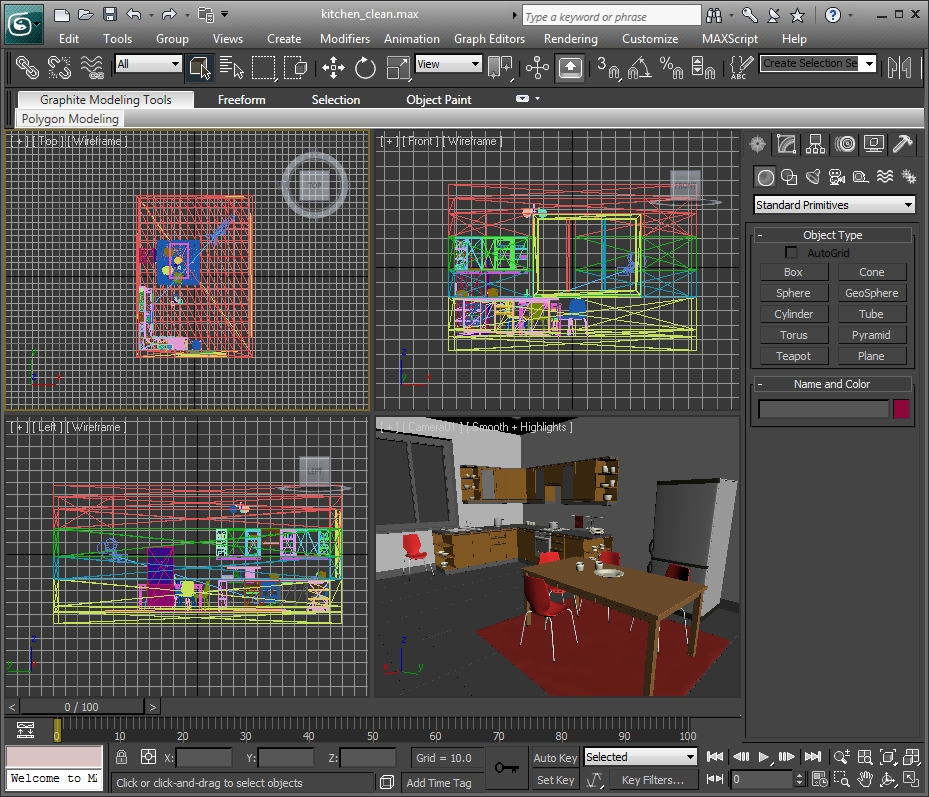
\includegraphics{images/import_1.jpg}}
\end{center}
Go to File$\to$Export$\to$Export, enter a filename for the exported scene and choose "Autodesk Collada (*.DAE)" as the target file type.
In the upcoming dialog, make sure that `Single Matrix' is disabled at the bottom -- otherwise your camera will face into the 
wrong direction (this is only an issue with Autodesk products).
\begin{center}
\scalebox{.4}{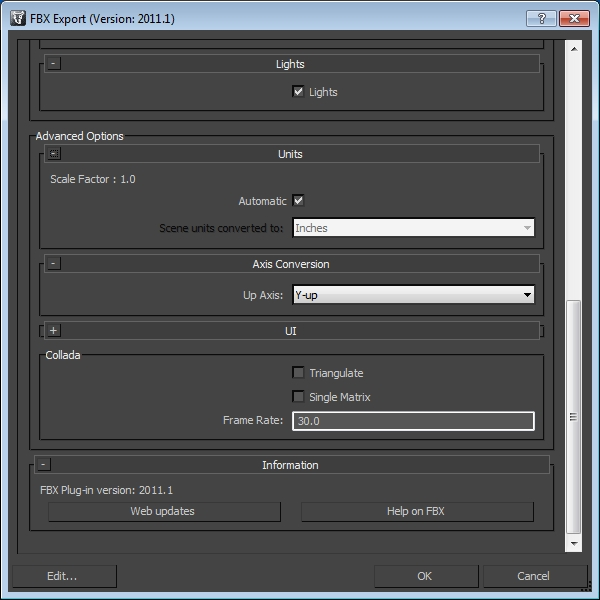
\includegraphics{images/import_2.jpg}}
\end{center}
Launch Mitsuba and select File$\to$Import. Next, open the exported DAE file by clicking on the topmost browse button and and change the color format to sRGB. The remaining options can be ignored for now.
\begin{center}
\scalebox{.5}{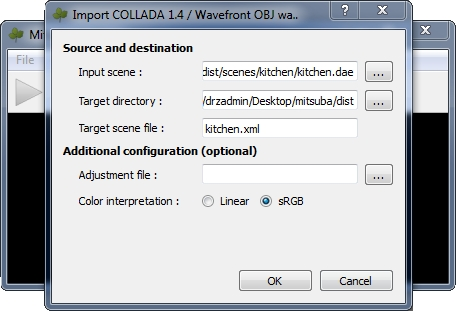
\includegraphics{images/import_3.jpg}}
\end{center}
After a moment, the scene will open -- rendering it in this form, e.g. using path tracing will produce an image like this:
\begin{center}
\scalebox{.5}{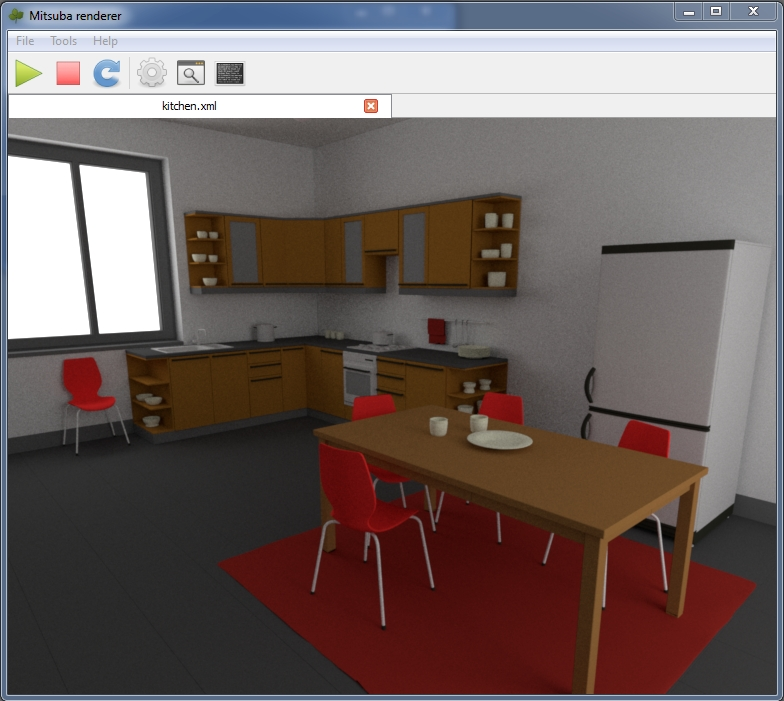
\includegraphics{images/import_4.jpg}}
\end{center}
Many of the materials in this rendering are incorrect, which is in part caused by the limited material description abilities of COLLADA.
To fix them, we will have to provide a so-called adjustment file. The idea here is very simple: if you look at the output file (\texttt{kitchen.xml}) 
generated by the conversion, you will notice that every relevant XML node has an \code{id} attribute. For instance, there is a material named \code{glass} with the following entry:
\begin{xml}
<bsdf id="glass" type="lambertian">
	<rgb name="reflectance" value="0.588235 0.588235 0.588235"/>
</bsdf>
\end{xml}
\newpage
This is the reason why the glass looks incorrect in the above rendering: it is completely diffuse!
To fix it, we will provide a dielectric material with the same \code{id} attribute, which then allows Mitsuba
to replace the incorrect material during import.
We can do this by creating a file named \code{kitchen\_adjustments.xml} containing
the following lines:
\begin{xml}
<adjustments>
	<bsdf id="glass" type="dielectric"/>
</adjustments>
\end{xml}
The adjustments mechanism can also be used to add content, such as light sources or even geometry. Insert the objects which should
be part part of the scene into the adjustment file, and they will be copied on every import. Replacement is not limited to materials -- it
can also be applied to the integrator or the camera -- you only make sure that the \code{id} fields match for the replacement to happen.
After tweaking the remaining materials in this fashion, it is possible to re-import the scene and this time specify the adjustment file in the import dialog.
This makes it possible to get the following more realistic result (material descriptions courtesy of Pomesuba):
\begin{center}
\scalebox{.5}{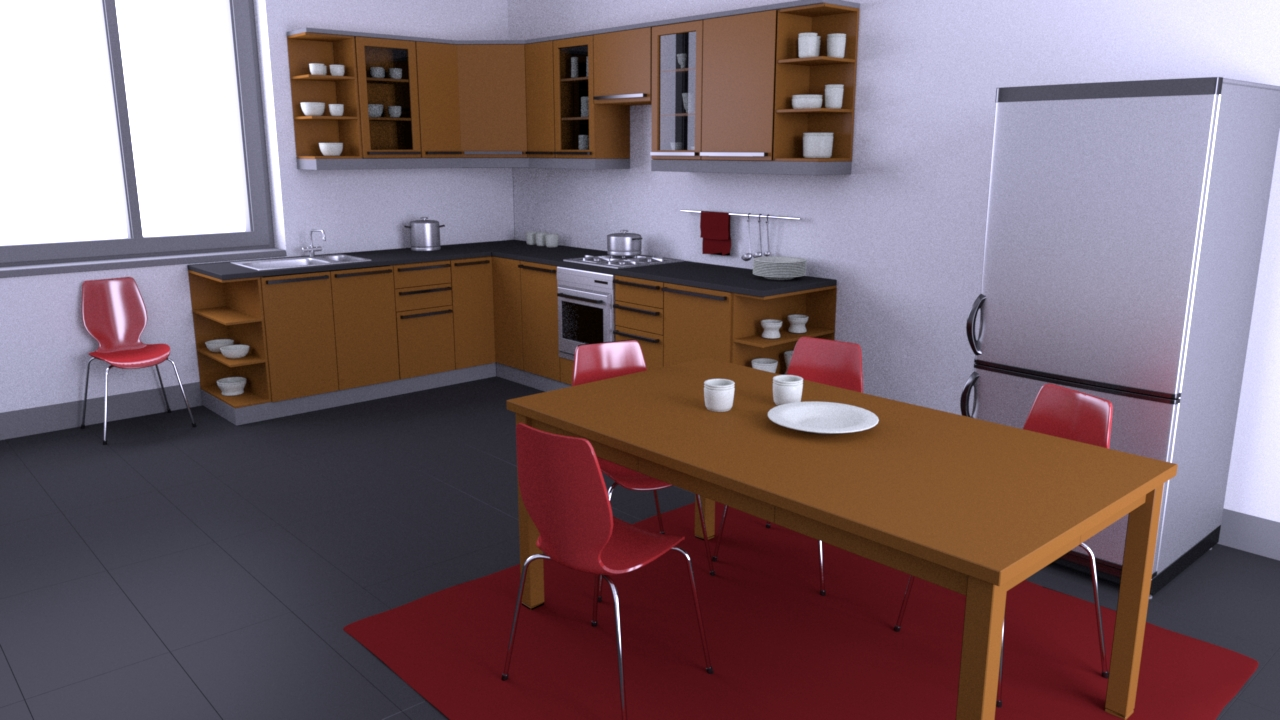
\includegraphics{images/import_5.jpg}}
\end{center}

%\part{Development guide}
\label{sec:development}
This chapter and the subsequent ones will provide an overview
of the coding conventions and general architecture of Mitsuba.
You should only read them if you wish to interface with the API
in some way (e.g. by developing your own plugins). The coding style
section is only relevant if you plan to submit patches that are meant
to become part of the main codebase.

\section{Code structure}
Mitsuba is split into four basic support libraries:
\begin{itemize}
\item The core library (\code{libcore}) implements basic functionality such as
    cross-platform file and bitmap I/O, data structures, scheduling, as well as logging and plugin management.
\item The rendering library (\code{librender}) contains abstractions
    needed to load and represent scenes containing  light sources, shapes, materials, and participating media.
\item The hardware acceleration library (\code{libhw})
    implements a cross-platform display library, an object-oriented OpenGL
    wrapper, as well as support for rendering interactive previews of scenes.
\item Finally, the bidirectional library (\code{libbidir})
    contains a support layer that is used to implement bidirectional rendering algorithms such as
    Bidirectional Path Tracing and Metropolis Light Transport.
\end{itemize}
A detailed reference of these APIs is available at
\url{http://www.mitsuba-renderer.org/api}. The next sections
present a few basic examples to get familiar with them.

\section{Coding style}
\paragraph{Indentation:} The Mitsuba codebase uses tabs for indentation,
which expand to \emph{four} spaces. Please make sure that you configure your editor
this way, otherwise the source code layout will look garbled.

\paragraph{Placement of braces:} Opening braces should be placed on the
same line to make the best use of vertical space, i.e.
\begin{cpp}
if (x > y) {
    x = y;
}
\end{cpp}

\paragraph{Placement of spaces:} Placement of spaces follows K\&R, e.g.
\begin{cpp}
if (x == y) {
    ..
} else if (x > y) {
    ..
} else {
    ..
}
\end{cpp}
rather than things like this
\begin{cpp}
if ( x==y ){
}
..
\end{cpp}

\paragraph{Name format:} Names are always written in camel-case.
Classes and structures start with a capital letter, whereas member functions
and attributes start with a lower-case letter. Attributes of classes
have the prefix \code{m\_}. Here is an example:
\begin{cpp}
class MyClass {
public:
    MyClass(int value) : m_value(value) { }

    inline void setValue(int value) { m_value = value; }
    inline int getValue() const { return m_value; }
private:
    int m_value;
};
\end{cpp}

\paragraph{Enumerations:} For clarity, both enumerations types and entries
start with a capital \textbf{E}, e.g.
\begin{cpp}
enum ETristate {
    ENo = 0,
    EYes,
    EMaybe
};
\end{cpp}
\paragraph{Constant methods and parameters:} Declare member functions and
their parameters as \code{const} whenever this is possible
and properly conveys the semantics.
\paragraph{Inline methods:} Always inline trivial pieces of code, such
as getters and setters.
\paragraph{Documentation:} Headers files should contain
Doxygen-compatible documentation. It is also a good idea to add
comments to a \code{.cpp} file to explain subtleties of an implemented algorithm.
However, anything pertaining to the API should go into the header file.

\paragraph{Boost:} Use the boost libraries whenever this helps to save
time or write more compact code.

\paragraph{Classes vs structures:}In Mitsuba, classes usually go onto the heap,
whereas structures may be allocated both on the stack and the heap.

Classes that derive from \code{Object} implement a protected virtual
deconstructor, which explicitly prevents them from being allocated on the stack.
The only way they can be deallocated is using the built-in reference
counting. This is done using the \code{ref<>} template, e.g.

\begin{cpp}
if (..) {
    ref<MyClass> instance = new MyClass();
    instance->doSomething()
}   // reference expires, instance will be deallocated
\end{cpp}

\paragraph{Separation of plugins:}Mitsuba encourages that plugins are only
used via the generic interface they implement. You will find that almost all plugins
(e.g. emitters) don't actually provide a header file, hence they can only be accessed
using the generic \code{Emitter} interface they implement. If any kind of special
interaction between plugins is needed, this is usually an indication that the
generic interface should be extended to accomodate this.

%\section{Designing a custom integrator plugin}
Suppose you want to design a custom integrator to render scenes in Mitsuba.
There are two general ways you can do this, and which one you should take
mostly depends on the characteristics of your particular integrator.

The framework distinguishes between \emph{sampling-based} integrators and 
\emph{generic} ones. A sampling-based integrator is able to generate 
(usually unbiased) estimates of the incident radiance along a specified rays, and this 
is done a large number of times to render a scene. A generic integrator
is more like a black box, where no assumptions are made on how the the image is
created. For instance, the VPL renderer uses OpenGL to rasterize the scene
using hardware acceleration, which certainly doesn't fit into the sampling-based pattern.
For that reason, it must be implemented as a generic integrator.

Generally, if you can package up your code to fit into the
\code{SampleIntegrator} interface, you should do it, because you'll get
parallelization and network rendering essentially for free. This is done
by transparently sending instances of your integrator class to all participating cores
and assigning small image blocks for each one to work on. Also, sampling-based
integrators can be nested within some other integrators, such as an
irradiance cache or an adaptive integrator. This cannot be done with generic
integrators due to their black-box nature. Note that it is often still 
possible to parallelize generic integrators, but this involves significantly 
more work.

In this section, we'll design a rather contrived sampling-based integrator, 
which renders a monochromatic image of your scene, where the intensity 
denotes the distance to the camera. But to get a feel for the overall 
framework, we'll start with an even simpler one, that just renders a 
solid-color image.

\subsection{Basic implementation}
In Mitsuba's \code{src/integrators} directory, create a file named 
\code{myIntegrator.cpp}. 

\begin{cpp}
#include <mitsuba/render/scene.h>

MTS_NAMESPACE_BEGIN

class MyIntegrator : public SampleIntegrator {
public:
	MTS_DECLARE_CLASS()
};

MTS_IMPLEMENT_CLASS_S(MyIntegrator, false, SampleIntegrator)
MTS_EXPORT_PLUGIN(MyIntegrator, "A contrived integrator");
MTS_NAMESPACE_END
\end{cpp}
The \code{scene.h} header file contains all of the dependencies we'll need
for now.
To avoid conflicts with other libraries, the whole framework is located in
a separate namespace named \code{mitsuba}, and the lines starting with 
\code{MTS\_NAMESPACE} ensure that our integrator is placed there
as well.

The two lines starting with \code{MTS\_DECLARE\_CLASS} and \code{MTS\_IMPLEMENT\_CLASS}
ensure that this class is recognized as a native Mitsuba class.
This is necessary to get things like run-time type information, reference counting,
and serialization/unserialization support. Let's take a look at the second of these
lines, because it contains several important pieces of information:

The suffix \code{S} in \code{MTS\_IMPLEMENT\_CLASS\_S} specifies that this is
a serializable class, which means that it can be sent over the network or 
written to disk and later restored. That also implies that certain methods
need to be provided by the implementation --- we'll add those in a moment.

The three following parameters specify the name of this class (\code{MyIntegrator}),
the fact that it is \emph{not} an abstract class (\code{false}), and the name of its
parent class (\code{SampleIntegrator}).

Just below, you can see a line that starts with
\code{MTS\_EXPORT\_PLUGIN}. As the name suggests, this line is only necessary
for plugins, and it ensures that the specified class (\code{MyIntegrator}) is 
what you want to be instantiated when somebody loads this plugin. It is also
possible to supply a short descriptive string.
\vspace{3mm}

Let's add an instance variable and a constructor:
\begin{cpp}
public:
    /// Initialize the integrator with the specified properties
    MyIntegrator(const Properties &props) : SampleIntegrator(props) {
        Spectrum defaultColor;
        defaultColor.fromLinearRGB(0.2f, 0.5f, 0.2f);
        m_color = props.getSpectrum("color", defaultColor);
    }

private:
	Spectrum m_color;
\end{cpp}

This code fragment sets up a default color (a light shade of green), which
can be overridden from the scene file. For example, one could instantiate
the integrator from an XML document like this

\begin{xml}
<integrator type="myIntegrator">
	<spectrum name="color" value="1.0"/>
</integrator>
\end{xml}
in which case white would take preference.
\vspace{3mm}

Next, we need to add serialization and unserialization support:
\begin{cpp}
    /// Unserialize from a binary data stream
    MyIntegrator(Stream *stream, InstanceManager *manager)
     : SampleIntegrator(stream, manager) {
        m_color = Spectrum(stream);
    }

    /// Serialize to a binary data stream
    void serialize(Stream *stream, InstanceManager *manager) const {
        SampleIntegrator::serialize(stream, manager);
        m_color.serialize(stream);
    }
\end{cpp}
This makes use of a \emph{stream} abstraction similar in style to Java. 
A stream can represent various things, such as a file, a console session, or a 
network communication link. Especially when dealing with multiple machines,
it is important to realize that the machines may use different binary representations
related to their respective \emph{endianness}. To prevent issues from arising,
the \code{Stream} interface provides many methods for writing and reading 
small chunks of data (e.g. \code{writeShort}, \code{readFloat}, ..),
which automatically perform endianness translation. In our case, the
\code{Spectrum} class already provides serialization/unserialization support,
so we don't really have to do anything.

Note that it is crucial that your code calls the serialization and unserialization 
implementations of the superclass!
We haven't used the \texttt{manager} parameter yet, so here is a quick overview
of what it does: if many cases, we don't just want to serialize a single class,
but a whole graph of objects. Some may be referenced many
times from different places, and potentially there are even cycles. If we just 
naively called the serialization and unserialization implementation of members 
recursively within each class, we'd waste much bandwitdth and potentially 
end up stuck in an infinite recursion.

This is where the instance manager comes in. Every time you want to serialize
a heap-allocated object (suppose it is of type \code{SomeClass}), 
instead of calling its serialize method, write

\begin{cpp}
ref<SomeClass> myObject = ...;
manager->serialize(stream, myObject.get());
\end{cpp}

Later, to unserialize the object from a stream again, write
\begin{cpp}
ref<SomeClass> myObject = static_cast<SomeClass *>(manager->getInstance(stream));
\end{cpp}

Behind the scenes, the object manager adds annotations to the data stream,
which ensure that you will end up with the exact same reference graph on the
remote side, while only one copy of every object is transmitted and no 
infinite recursion can occur. But we digress -- let's go back to our integrator.
\vspace{3mm}

The last thing to add is a function, which returns an estimate for the
radiance along a ray differential: here, we simply return the stored color
\begin{cpp}
    /// Query for an unbiased estimate of the radiance along <tt>r</tt>
   Spectrum Li(const RayDifferential &r, RadianceQueryRecord &rRec) const {
       return m_color;
   }
\end{cpp}

Let's try building the plugin: edit the \code{SConstruct} file in the main
directory, and add the following line after the comment ''\code{\# Integrators}'':
\begin{cpp}
plugins += env.SharedLibrary('plugins/myIntegrator', ['src/integrators/myIntegrator.cpp'])
\end{cpp}
After calling, \texttt{scons}, you should be able to use your new integrator
in parallel rendering jobs and you'll get something like this:
\begin{center}
\scalebox{.4}{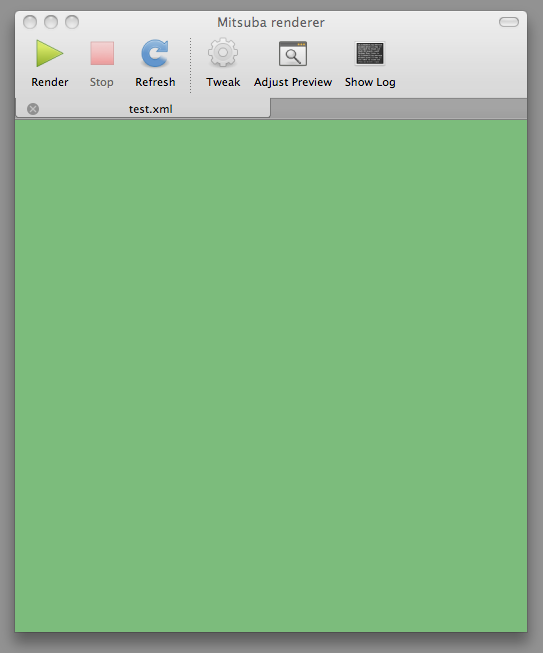
\includegraphics{images/integrator_green.png}}
\end{center}
That is admittedly not very exciting --- so let's do some actual computation.
\subsection{Visualizing depth}
Add an instance variable \code{Float m\_maxDist;} to the implementation. This
will store the maximum distance from the camera to any object, which is needed
to map distances into the $[0,1]$ range. Note the upper-case \code{Float} --- 
this means that either a single- or a double-precision variable is 
substituted based the compilation flags. This variable constitutes local
state, thus it must not be forgotten in the serialization- and unserialization routines:
append
\begin{cpp}
	m_maxDist = stream->readFloat();
\end{cpp}
and
\begin{cpp}
	stream->writeFloat(m_maxDist);
\end{cpp}
to the unserialization constructor and the \code{serialize} method, respectively.

We'll conservatively bound the maximum distance by measuring the
distance to all corners of the bounding box, which encloses the scene.
To avoid having to do this every time \code{Li()} is called,
we can override the \code{preprocess} function:
\begin{cpp}
	/// Preprocess function -- called on the initiating machine
	bool preprocess(const Scene *scene, RenderQueue *queue, 
			const RenderJob *job, int sceneResID, int cameraResID, 
			int samplerResID) {
		SampleIntegrator::preprocess(scene, queue, job, sceneResID, 
			cameraResID, samplerResID);

		const AABB &sceneAABB = scene->getAABB();
		Point cameraPosition = scene->getCamera()->getPosition();
		m_maxDist = - std::numeric_limits<Float>::infinity();

		for (int i=0; i<8; ++i)
			m_maxDist = std::max(m_maxDist, 
				(cameraPosition - sceneAABB.getCorner(i)).length());

		return true;
	}
\end{cpp}
The bottom of this function should be relatively self-explanatory. The
numerous arguments at the top are related to the parallelization layer, which will be
considered in more detail in the next section. Briefly, the render queue
provides synchronization facilities for render jobs (e.g. one can wait
for a certain job to terminate). And the integer parameters are
global resource identifiers. When a network render job runs, many associated
pieces of information (the scene, the camera, etc.) are wrapped into global resource chunks
shared amongst all nodes, and these can be referenced using such identifiers.

One important aspect of the \code{preprocess} function is that it is executed 
on the initiating node and before any of the parallel rendering begins. 
This can be used to compute certain things only once. Any
information updated here (such as \code{m\_maxDist}) will be forwarded to the
other nodes before the rendering begins.

Now, replace the body of the \code{Li} method with 
\begin{cpp}
	if (rRec.rayIntersect(r)) {
		Float distance = rRec.its.t;
		return Spectrum(1.0f - distance/m_maxDist) * m_color;
	}
	return Spectrum(0.0f);
\end{cpp}
and the distance renderer is done!
\begin{center}
\scalebox{.3}{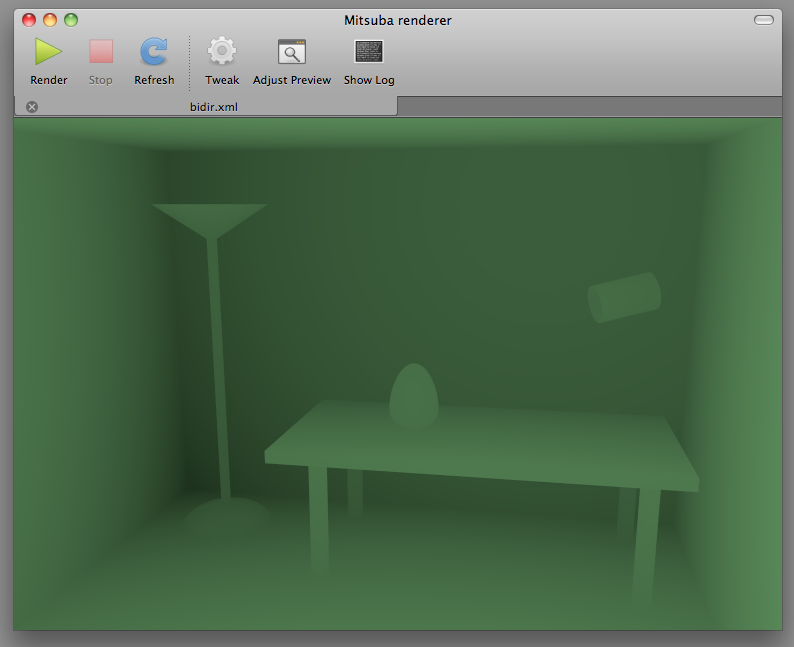
\includegraphics{images/integrator_depth.png}}
\end{center}
There are a few more noteworthy details: first of all, the ``usual'' way
to intersect a ray against the scene actually works like this:
\begin{cpp}
	Intersection its;
	Ray ray = ...;
	if (scene->rayIntersect(ray, its)) {
		/* Do something with the intersection stored in 'its' */
	}
\end{cpp}
As you can see, we did something slightly different in the distance 
renderer fragment above (we called \code{RadianceQueryRecord::rayIntersect()}
on the supplied parameter \code{rRec}), and the reason for this is \emph{nesting}.
\subsection{Nesting}
The idea of of nesting is that sampling-based rendering techniques can be
embedded within each other for added flexibility: for instance, one 
might concoct a  1-bounce indirect rendering technique complete with 
irradiance caching and adaptive integration simply by writing the following 
into a scene XML file:
\begin{xml}
<!-- Adaptively integrate using the nested technique -->
<integrator type="errctrl"> 
	<!-- Irradiance caching + final gathering with the nested technique -->
	<integrator type="irrcache"> 
		<!-- Simple direct illumination technique -->
		<integrator type="direct"> 
	</integrator>
</integrator>
\end{xml}
To support this kind of complex interaction, some information needs to be passed between the 
integrators, and the \code{RadianceQueryRecord} parameter of the function
\code{SampleIntegrator::Li} is used for this.

This brings us back to the odd way of computing an intersection a moment ago: 
the reason why we didn't just do this by calling  
\code{scene->rayIntersect()} is that our technique might actually be nested
within a parent technique, which has already computed this intersection.
To avoid wasting resources, the function \code{rRec.rayIntersect} first 
determines whether an intersection record has already been provided. 
If yes, it does nothing. Otherwise, it takes care of computing one. 

The radiance query record also lists the particular \emph{types} of radiance requested
by the parent integrator -- your implementation should respect these as much
as possible. Your overall code might for example be structured like this:

\begin{cpp}
   Spectrum Li(const RayDifferential &r, RadianceQueryRecord &rRec) const {
	  Spectrum result;
      if (rRec.type & RadianceQueryRecord::EEmittedRadiance) {
         // Emitted surface radiance contribution was requested
		 result += ...;
	  }
      if (rRec.type & RadianceQueryRecord::EDirectRadiance) {
         // Direct illumination contribution was requested
		 result += ...;
	  }
	  ...
	  return result;
   }
\end{cpp}

%\section{Parallelization layer}
Mitsuba is built on top of a flexible parallelization layer, which spreads out
various types of computation over local and remote cores.
The guiding principle is that if an operation can potentially take longer than a
few seconds, it ought to use all the cores it can get.

Here, we will go through a basic example, which will hopefully provide sufficient intuition
to realize more complex tasks. 
To obtain good (i.e. close to linear) speedups, the parallelization layer depends on
several key assumptions of the task to be parallelized:
\begin{itemize}
\item The task can easily be split up into a discrete number of \emph{work units}, which requires a negligible amount of computation.
\item Each work unit is small in footprint so that it can easily be transferred over the network or shared memory. 
\item A work unit constitutes a significant amount of computation, which by far outweighs the cost of transmitting it to another node.
\item The \emph{work result} obtained by processing a work unit is again small in footprint, so that it can easily be transferred back.
\item Merging all work results to a solution of the whole problem requires a negligible amount of additional computation.
\end{itemize}
This essentially corresponds to a parallel version of \emph{Map} (one part of \emph{Map\&Reduce}) and is 
ideally suited for most rendering workloads. 

The example we consider here computes a \code{ROT13} ``encryption'' of a string, which 
most certainly violates the ``significant amount of computation'' assumption.
It was chosen due to the inherent parallelism and simplicity of this task.
While of course over-engineered to the extreme, the example hopefully 
communicates how this framework might be used in more complex scenarios.

We will implement this program as a plugin for the utility launcher \code{mtsutil}, which
frees us from having to write lots of code to set up the framework, prepare the
scheduler, etc.

We start by creating the utility skeleton file \code{src/utils/rot13.cpp}:
\begin{cpp}
#include <mitsuba/render/util.h>

MTS_NAMESPACE_BEGIN

class ROT13Encoder : public Utility {
public:
	ROT13Encoder(UtilityServices *us) : Utility(us) { }

	int run(int argc, char **argv) {
		cout << "Hello world!" << endl;
		return 0;
	}

	MTS_DECLARE_CLASS()
};

MTS_IMPLEMENT_CLASS(ROT13Encoder, false, Utility)
MTS_EXPORT_UTILITY(ROT13Encoder, "Perform a ROT13 encryption of a string")
MTS_NAMESPACE_END
\end{cpp}
The file must also be added to the build system: insert the line
\begin{shell}
plugins += $\texttt{env}$.SharedLibrary('plugins/rot13', ['src/utils/rot13.cpp'])
\end{shell}
into the SConscript (near the comment ``\code{Build the plugins -- utilities}''). After compiling
using \code{scons}, the \code{mtsutil} binary should automatically pick up your new utility plugin:
\begin{shell}
$\texttt{\$}$ mtsutil
..
The following utilities are available:

	addimages             Generate linear combinations of EXR images
	rot13                 Perform a ROT13 encryption of a string
\end{shell}
It can be executed as follows:
\begin{shell}
$\texttt{\$}$ mtsutil rot13
2010-08-16 18:38:27 INFO  main [src/mitsuba/mtsutil.cpp:276] Mitsuba version 0.1.1, Copyright (c) 2010 Wenzel Jakob
2010-08-16 18:38:27 INFO  main [src/mitsuba/mtsutil.cpp:350] Loading utility "rot13" ..
Hello world!
\end{shell}

Our approach for implementing distributed ROT13 will be to treat each character as an 
indpendent work unit. Since the ordering is lost when sending out work units, we must
also include the position of the character in both the work units and the work results.

All of the relevant interfaces are contained in \code{include/mitsuba/core/sched.h}.
For reference, here are the interfaces of \code{WorkUnit} and \code{WorkResult}:
\newpage
\begin{cpp}
/**
 * Abstract work unit. Represents a small amount of information
 * that encodes part of a larger processing task. 
 */
class MTS_EXPORT_CORE WorkUnit : public Object {
public:
	/// Copy the content of another work unit of the same type
	virtual void set(const WorkUnit *workUnit) = 0;

	/// Fill the work unit with content acquired from a binary data stream
	virtual void load(Stream *stream) = 0;

	/// Serialize a work unit to a binary data stream
	virtual void save(Stream *stream) const = 0;

	/// Return a string representation
	virtual std::string toString() const = 0;

	MTS_DECLARE_CLASS()
protected:
	/// Virtual destructor
	virtual ~WorkUnit() { }
};
/**
 * Abstract work result. Represents the information that encodes 
 * the result of a processed <tt>WorkUnit</tt> instance.
 */
class MTS_EXPORT_CORE WorkResult : public Object {
public:
	/// Fill the work result with content acquired from a binary data stream
	virtual void load(Stream *stream) = 0;

	/// Serialize a work result to a binary data stream
	virtual void save(Stream *stream) const = 0;

	/// Return a string representation
	virtual std::string toString() const = 0;

	MTS_DECLARE_CLASS()
protected:
	/// Virtual destructor
	virtual ~WorkResult() { }
};
\end{cpp}
\newpage
In our case, the \code{WorkUnit} implementation then looks like this:
\begin{cpp}
class ROT13WorkUnit : public WorkUnit {
public:
	void set(const WorkUnit *workUnit) {
		const ROT13WorkUnit *wu = 
			static_cast<const ROT13WorkUnit *>(workUnit);
		m_char = wu->m_char;
		m_pos = wu->m_pos;
	}

	void load(Stream *stream) {
		m_char = stream->readChar();
		m_pos = stream->readInt();
	}
	
	void save(Stream *stream) const {
		stream->writeChar(m_char);
		stream->writeInt(m_pos); 
	}

	std::string toString() const {
		std::ostringstream oss;
		oss << "ROT13WorkUnit[" << endl
			<< "  char = '" << m_char << "'," << endl
			<< "  pos = " << m_pos << endl
			<< "]";
		return oss.str();
	}

	inline char getChar() const { return m_char; }
	inline void setChar(char value) { m_char = value; }
	inline int getPos() const { return m_pos; }
	inline void setPos(int value) { m_pos = value; }

	MTS_DECLARE_CLASS()
private:
	char m_char;
	int m_pos;
};

MTS_IMPLEMENT_CLASS(ROT13WorkUnit, false, WorkUnit)
\end{cpp}
The \code{ROT13WorkResult} implementation is not reproduced since it is almost identical 
(except that it doesn't need the \code{set} method).
The similarity is not true in general: for most algorithms, the work unit and result 
will look completely different.

Next, we need a class, which does the actual work of turning a work unit into a work result
(a subclass of \code{WorkProcessor}). Again, we need to implement a range of support
methods to enable the various ways in which work processor instances will be submitted to 
remote worker nodes and replicated amongst local threads.
\begin{cpp}
class ROT13WorkProcessor : public WorkProcessor {
public:
	/// Construct a new work processor
	ROT13WorkProcessor() : WorkProcessor() { }

	/// Unserialize from a binary data stream (nothing to do in our case)
	ROT13WorkProcessor(Stream *stream, InstanceManager *manager)
		: WorkProcessor(stream, manager) { }

	/// Serialize to a binary data stream (nothing to do in our case)
	void serialize(Stream *stream, InstanceManager *manager) const {
	}

	ref<WorkUnit> createWorkUnit() const {
		return new ROT13WorkUnit();
	}

	ref<WorkResult> createWorkResult() const { 
		return new ROT13WorkResult();
	}

	ref<WorkProcessor> clone() const {
		return new ROT13WorkProcessor(); // No state to clone in our case
	}

	/// No internal state, thus no preparation is necessary
	void prepare() { }

	/// Do the actual computation
	void process(const WorkUnit *workUnit, WorkResult *workResult, 
				 const bool &stop) {
		const ROT13WorkUnit *wu 
			= static_cast<const ROT13WorkUnit *>(workUnit);
		ROT13WorkResult *wr = static_cast<ROT13WorkResult *>(workResult);
		wr->setPos(wu->getPos());
		wr->setChar((std::toupper(wu->getChar()) - 'A' + 13) % 26 + 'A');
	}
	MTS_DECLARE_CLASS()
};
MTS_IMPLEMENT_CLASS_S(ROT13WorkProcessor, false, WorkProcessor)
\end{cpp}
Since our work processor has no state, most of the implementations
are rather trivial. Note the \code{stop} field in the \code{process}
method. This field is used to abort running jobs at the users requests, hence
it is a good idea to periodically check its value during lengthy computations.

Finally, we need a called \emph{parallel process}
instance, which is responsible for creating work units and stitching
work results back into a solution of the whole problem. The \code{ROT13}
implementation might look as follows:
\begin{cpp}
class ROT13Process : public ParallelProcess {
public:
	ROT13Process(const std::string &input) : m_input(input), m_pos(0) {
		m_output.resize(m_input.length());
	}

	ref<WorkProcessor> createWorkProcessor() const {
		return new ROT13WorkProcessor();
	}

	std::vector<std::string> getRequiredPlugins() {
		std::vector<std::string> result;
		result.push_back("rot13");
		return result;
	}

	EStatus generateWork(WorkUnit *unit, int worker /* unused */) {
		if (m_pos >= (int) m_input.length())
			return EFailure;
		ROT13WorkUnit *wu = static_cast<ROT13WorkUnit *>(unit);

		wu->setPos(m_pos);
		wu->setChar(m_input[m_pos++]);

		return ESuccess;
	}

	void processResult(const WorkResult *result, bool cancelled) {
		if (cancelled) // indicates a work unit, which was 
			return;    // cancelled partly through its execution
		const ROT13WorkResult *wr = 
			static_cast<const ROT13WorkResult *>(result);
		m_output[wr->getPos()] = wr->getChar();
	}

	inline const std::string &getOutput() {
		return m_output;
	}

	MTS_DECLARE_CLASS()
public:
	std::string m_input;
	std::string m_output;
	int m_pos;
};
MTS_IMPLEMENT_CLASS(ROT13Process, false, ParallelProcess)
\end{cpp}
The \code{generateWork} method produces work units until we have moved past
the end of the string, after which it returns the status code \code{EFailure}.
Note the method \code{getRequiredPlugins()}: this is necessary to use 
the utility across
machines. When communicating with another node, it ensures that the remote side
loads the \code{ROT13*} classes at the right moment.

To actually use the \code{ROT13} encoder, we must first launch the newly created parallel process
from the main utility function (the `Hello World' code we wrote earlier). We can adapt it as follows:
\begin{cpp}
	int run(int argc, char **argv) {
		if (argc < 2) {
			cout << "Syntax: mtsutil rot13 <text>" << endl;
			return -1;
		}

		ref<ROT13Process> proc = new ROT13Process(argv[1]);
		ref<Scheduler> sched = Scheduler::getInstance();

		/* Submit the encryption job to the scheduler */
		sched->schedule(proc);

		/* Wait for its completion */
		sched->wait(proc);

		cout << "Result: " << proc->getOutput() << endl;

		return 0;
	}
\end{cpp}
After compiling everything using \code{scons}, an exemplary usage
would be to encode a string (e.g. \code{SECUREBYDESIGN}), while 
forwarding all computation to a network machine. (\code{-p0} disables
all local worker threads). Adding a verbose flag (\code{-v}) shows 
some additional scheduling information:
\begin{shell}
$\texttt{\$}$ mtsutil -vc feynman -p0 rot13 SECUREBYDESIGN
2010-08-17 01:35:46 INFO  main [src/mitsuba/mtsutil.cpp:201] Mitsuba version 0.1.1, Copyright (c) 2010 Wenzel Jakob
2010-08-17 01:35:46 INFO  main [SocketStream] Connecting to "feynman:7554"
2010-08-17 01:35:46 DEBUG main [Thread] Spawning thread "net0_r"
2010-08-17 01:35:46 DEBUG main [RemoteWorker] Connection to "feynman" established (2 cores).
2010-08-17 01:35:46 DEBUG main [Scheduler] Starting ..
2010-08-17 01:35:46 DEBUG main [Thread] Spawning thread "net0"
2010-08-17 01:35:46 INFO  main [src/mitsuba/mtsutil.cpp:275] Loading utility "rot13" ..
2010-08-17 01:35:46 DEBUG main [Scheduler] Scheduling process 0: ROT13Process[unknown]..
2010-08-17 01:35:46 DEBUG main [Scheduler] Waiting $\texttt{for}$ process 0
2010-08-17 01:35:46 DEBUG net0 [Scheduler] Process 0 has finished generating work
2010-08-17 01:35:46 DEBUG net0_r[Scheduler] Process 0 is $\texttt{complete}$.
Result: FRPHEROLQRFVTA
2010-08-17 01:35:46 DEBUG main [Scheduler] Pausing ..
2010-08-17 01:35:46 DEBUG net0 [Thread] Thread "net0" has finished
2010-08-17 01:35:46 DEBUG main [Scheduler] Stopping ..
2010-08-17 01:35:46 DEBUG main [RemoteWorker] Shutting down
2010-08-17 01:35:46 DEBUG net0_r[Thread] Thread "net0_r" has finished
\end{shell}
\subsection{Global Resources}
TBD.

\section{Acknowledgments}
I am indebted to my advisor Steve Marschner for allowing me to devote
a significant amount of my research time to this project. His insightful and
encouraging suggestions have helped transform this program into much more than
I ever thought it would be.

The architecture of Mitsuba as well as some individual components are based on
implementations discussed in: \emph{Physically Based Rendering - From Theory
To Implementation} by Matt Pharr and Greg Humphreys.

Some of the GUI icons were taken from the Humanity icon set by Canonical Ltd.
The material test scene was created by Jonas Pilo, and the environment map
it uses is courtesy of Bernhard Vogl.

The included index of refraction data files for conductors are copied from
PBRT. They are originally from the Luxpop database (\url{www.luxpop.com})
and are based on data by Palik et al. \cite{Palik1998Handbook}
and measurements of atomic scattering factors made by the Center For
X-Ray Optics (CXRO) at Berkeley and the Lawrence Livermore National
Laboratory (LLNL).

The following people have kindly contributed code or bugfixes:
\begin{itemize}
\item Milo\^{s} Ha\^{s}an
\item Marios Papas
\item Edgar Vel\'{a}zquez-Armend\'{a}riz
\item Jirka Vorba
\item Leonhard Gr\"unschlo\ss
\end{itemize}

Mitsuba makes heavy use of the following amazing libraries and tools:
\begin{itemize}
\item Qt 4 by Digia
\item OpenEXR by Industrial Light \& Magic
\item Xerces-C+\!+ by the Apache Foundation
\item Eigen by Beno\^it Jacob and Ga\"el Guennebaud
\item SSE math functions by Julien Pommier
\item The Boost C+\!+ class library
\item GLEW by Milan Ikits, Marcelo E. Magallon and Lev Povalahev
\item Mersenne Twister by Makoto Matsumoto and Takuji Nishimura
\item Cubature by Steven G. Johnson
\item COLLADA DOM by Sony Computer Entertainment
\item libjpeg-turbo by Darrell Commander and others
\item libpng by Guy Eric Schalnat, Andreas Dilger, Glenn Randers-Pehrson and \mbox{others}
\item libply by Ares Lagae
\item BWToolkit by Brandon Walkin
\item The SCons build system by the SCons Foundation
\end{itemize}


\bibliographystyle{acm}
\bibliography{main}

\end{document}
